\chapter{Convolutional Neural Network}
\textbf{Convolutional Neural Network} (CNN) are particular types of neural network
feed forward. Their goal is to use multiple layers, stacked one on top of the other,
in order to extract input-related features. These layers are organized in a
hierarchical way, where the lower level calculates more global feature that can
be used in another task, while higher layer learns more specific features related
to the task.

Unlike the networks seen so far, CNNs organize weights using 3 dimensions as shown
in Figure \ref{fig:weights}. From this point on, we will talk about the weights
also considering the \textbf{volume}. These volumes arise because the input
consists of spatial dimensions (image width and height) along with multiple input
channels (e.g., RGB for color images).

\begin{figure}[!ht]
    \centering
    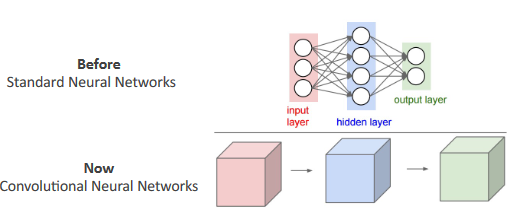
\includegraphics[width=0.5\textwidth]{img/CNN/weights.png}
    \caption{Weights representation in Feed Forward vs CNN.}
    \label{fig:weights}
\end{figure}

In a CNN each neuron acts as a filter, processing the entire spatial dimensions
and all input channels simultaneously. The output of each layer is another volume,
where the depth corresponds to the number of filters (or neurons) in the hidden
layer.

This particular type of network is widely used in the field of digital signal
processing, such as image or audio signals. If we look at image processing, this
kind of neural network offers a much more cost-effective approach than traditional
feed forward.

The most significant difference lies in how connections are structured. In a
traditional feed forward network, each input neuron is fully connected to all
neurons in the next layer. This results in a significant complexity challenge.
For instance, with an image of $100 \times 100$ pixels, the input to the network
is a vector of $10000$ pixels, leading to an enormous number of connections.

CNNs, on the other hand, introduce local connectivity, where each neuron focuses
on a small, localized portion of the image in each channel (\textbf{Local
    connectivity}) as shown in Figure \ref{fig:localConn}.

\begin{figure}[!ht]
    \centering
    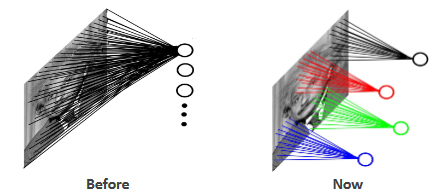
\includegraphics[width=0.45\linewidth]{img/CNN/localConn.png}
    \caption{Difference between the connections of neurons in a feed forward
        network and a CNN.}
    \label{fig:localConn}
\end{figure}

This drastically reduces the number of neurons and connections required. For
example, if the input image has dimensions $1000 \times 1000 \times 3$ (width,
height, and 3 color channels), a single neuron could use a $5 \times 5 \times 3 = 75$
parameters. This is because the neuron processes a $5 \times 5$ spatial region
across all channels of the previous layer, a property referred to as \textbf{full
    depth} connectivity.

Also, another difference is that now, we have neurons organized in depth, we have
multiple neurons all looking the same region of the input volume, stacked along depth
dimension. This is shown in Figure \ref{fig:depth}.

\begin{figure}[!ht]
    \centering
    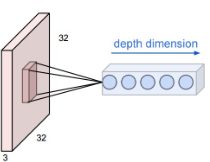
\includegraphics[width=0.25\linewidth]{img/CNN/depth.png}
    \caption{Organization of neurons in CNN}
    \label{fig:depth}
\end{figure}

In total we have $5\times 5\times 3$ weights to learn shared between each patch
of the image, this reduce a lot the number of learning parameter compared to
feed forward network. This concept is called \textbf{weights sharing}, which means
that the weights in the layer are shared across spatial positions.

In general, the structure of a CNN is organized so that it has a first part,
which includes convolutional layers, that extract the main characteristics from
the input. There is then a second part, composed of fully connected layer, which
performs the actual classification task. We can then represent this type of
network with a structure like the one shown in Figure \ref{fig:cnnarc}.

\begin{figure}[!ht]
    \centering
    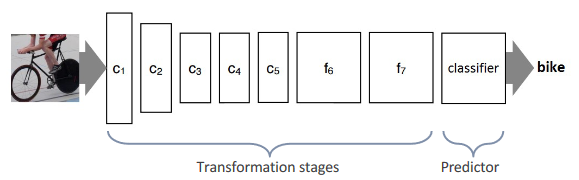
\includegraphics[width=\linewidth]{img/CNN/CNNarc.png}
    \caption{Overall CNN architecture.}
    \label{fig:cnnarc}
\end{figure}

The concept of \textbf{backpropagation} can still be utilized with this
architecture, which is a crucial aspect of training CNNs.

Respect to traditional neural networks, CNNs incorporate additional specialized
layers, such as \textbf{Spatial pooling} and \textbf{Local response normalization}.

These layers are useful to reduce computational complexity, increase invariance
and ease the optimization.
\section{CNNs components}
\subsection{Linear Convolution}
We begin by introducing the concept behind convolutional networks, namely the
concept of \textbf{linear convolution}. Convolution is a linear, local
(it applies on patches) and translation-invariant operator. To enrich the data
representation, we can use a \textbf{filter bank}, that is a collection of $Q$
sets of $K$ filters that allows to produce an output of $Q$ channel.

Let's see now, on a more mathematical level, what convolution represents. First we
introduce what we need:
\begin{itemize}
    \item $x = H \times W \times K$ is our input where $H$ represents the height
          dimension, $W$ the width dimension and $K$ the number of channels.
    \item $F = H' \times W' \times K \times Q$ is our filter bank where $Q$ is
          the number of filters that need to be apply to each channel.
    \item $y = (H - H' + 1) \times (W - W' + 1) \times Q$ is our output.
\end{itemize}

In addition to these, another very important thing to define is the \textbf{stride}.
The stride determines the step size for moving the filter across the input. By
default, the stride is set to 1, meaning the filter's center moves one pixel at
a time before being applied again.

\begin{note}
    A filter bank with 16 filters of depth $K$ produces an output with 16 channels.
\end{note}

The convolution is expressed by the following formula:
\begin{equation}
    y_{i, j, q} = y_q + \sum_{u = 0}^{H - 1}\sum_{v = 0}^{W - 1}\sum_{k = 1}^{K} x_{u + i, v + j, k} \cdot F_{u, v, k, q}
\end{equation}
where:
\begin{itemize}
    \item $y_q$ is the bias of the filter $F_q$;
    \item $x_{u + i, v + j, k}$ is the input patch of channel $k$;
    \item $F_{u, v, k, q}$ is the filter for the channel $k$ that computes output
          channel $q$.
\end{itemize}

\begin{figure}[!ht]
    \centering
    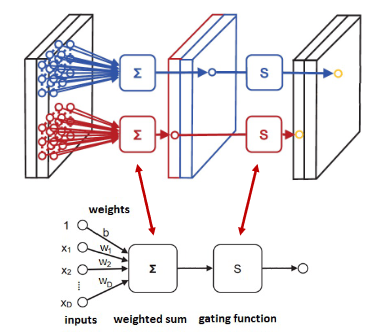
\includegraphics[width=0.25\linewidth]{img/CNN/Conv2Filter.png}
    \caption{Example of convolutional network with a filter bank of two elements.}
    \label{fig:conv2filter}
\end{figure}

We can apply filters in 2 way:
\begin{itemize}
    \item \textbf{Lattice structure}: a single filter is applied to a single
          channel ($K = 1$);
    \item \textbf{Multiple feature structure}: a single filter is applied to all
          channel of the input image $(K > 1)$.
\end{itemize}

In CNN, after the filter application we use a non-linear activation function,
also called \textbf{gating function}: \textit{Sigmoid}, \textit{Tanh}, \textit{ReLU}
and \textit{SmoothReLU}.

\subsection{Spatial pooling}
We have already said that there are different types of layers in a CNN, one of
them is the \textbf{spatial pooling}.

The purpose of this layer is to subsample the image, reducing its spatial
dimensions and, in turn, the computational load. Additionally, spatial pooling
aggregates information from the image, enhancing translation invariance, which
makes the model more robust to variations in the exact spatial positions of
features. This is done in two main ways:
\begin{itemize}
    \item \textbf{avg pooling}: computing an average of the value of the pixels
          in the neighborhood:
          \begin{equation}
              y_{ijk} =\text{avg}_{p, q \in \Omega} x_{p, q, k}
          \end{equation}
    \item \textbf{max pooling}: taking the maximum value from the pixels in the
          neighborhood:
          \begin{equation}
              y_{ijk} = \max_{p, q \in \Omega_{i, j}} x_{p, q, k}
          \end{equation}
\end{itemize}

This is done channel by channel.
\subsection{Local Response Normalization}
\textbf{Local Response Normalization} layers have the objective of normalizing the
effect of contrast to improve the network invariance in this respect. This layer
also allows for improved optimization and sparsity (accuracy and speed).

In general, there are two ways of applying it:
\begin{itemize}
    \item \textbf{Within Channel}: operates independently on different feature
          channels, and also rescales each input feature basing on a local
          neighborhood.
          \begin{equation}
              y_{i, j, k} = x_{i, j, k} \left(k + \alpha \sum_{(u, v) \in \mathcal{N}(i, j)} x_{u, v, k}^2 \right)^{-\beta}
          \end{equation}
    \item \textbf{Across Channels}: operates independently at each spatial location
          and groups of channels. It also normalizes groups $G(k)$ of feature
          channels. Groups are usually defined in a sliding window manner.
          \begin{equation}
              y_{i, j, k} = x_{i, j, k} \left(k + \alpha \sum_{q \in G(k)} x_{i, j, q}^2 \right)^{-\beta}
          \end{equation}
\end{itemize}

\subsection{Input sensibility}
CNN are sensible to the input images, moreover we need a lot of data to train
from scratch a CNN. So we have to normalize images using:
\begin{itemize}
    \item \textbf{Local mean subtraction}
    \item \textbf{Normalization}
\end{itemize}
to have data centered in 0. To prevent overfitting we can use:
\begin{itemize}
    \item Weight decay;
    \item Dropout;
    \item Data augmentation: for example changing illuminants, flip the image,
          random crop and a geometric distortion.
\end{itemize}
Remember that is always better to accept new data.

\section{CNN Architectures}
Below, we will introduce some of the most famous CNN architectures. This is done
because the training from zero of one of these models requires a very large amount
of data and many computational resources.
\begin{itemize}
    \item \textbf{LeNet} is one of the first model that this is first create for
          the MNIST dataset. This network take in input a gray scale image of
          size $32 \times 32$.
          \begin{figure}[!ht]
              \centering
              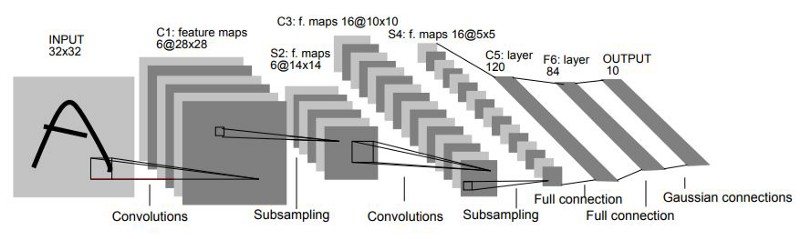
\includegraphics[width=0.4\linewidth]{img/CNN/LeNet-5.jpeg}
              \caption{LeNet}
              \label{fig:lenet}
          \end{figure}
    \item \textbf{AlexNet} was created for the ImageNet challenge and combines
          some convolutional layers with feed forward layers. It starts with a
          large convolutional level that is gradually reduced in order to encode
          the deeper layers of the more specific information in the task. In
          general we decrease filter dimension, increasing the depth channels.
          \begin{figure}[!ht]
              \centering
              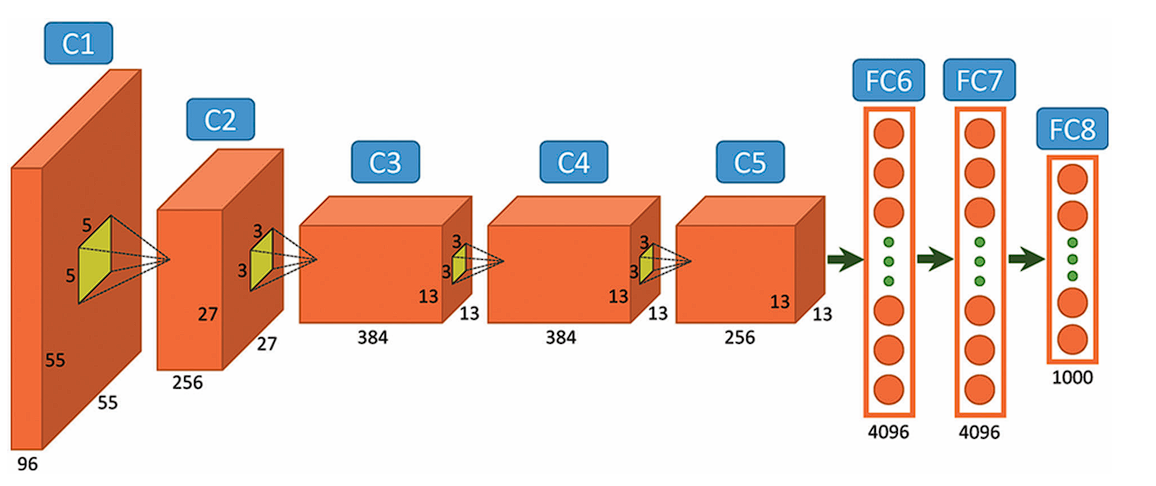
\includegraphics[width=0.4\linewidth]{img/CNN/alexNet.png}
              \caption{AlexNet}
              \label{fig:alexnet}
          \end{figure}
    \item \textbf{VGG} is a family of CNNs that consists of networks with varying
          numbers of convolutional layers. Compared to AlexNet, VGG uses smaller
          filters to reduce the number of parameters. Additionally, due to the
          concept of the \textbf{receptive field}, using smaller filters in multiple
          layers can achieve a similar receptive field to using a larger filter
          in a single layer. This allows VGG to maintain model depth while managing
          the number of parameters more efficiently.
          \begin{figure}[!ht]
              \centering
              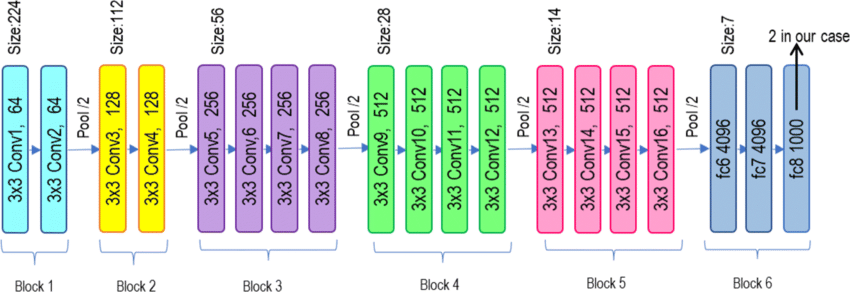
\includegraphics[width=0.4\linewidth]{img/CNN/VGG.png}
              \caption{VGG-19}
              \label{fig:vgg}
          \end{figure}
    \item \textbf{GoogLeNet} is one of the first networks to introduce the
          \textbf{module} concept. In particular, it uses the module called
          \textbf{inception} which is a part of the network, which can be stacked
          over other similar modules to get a larger network.

          As we are increasing the size of the network, we may encounter the
          problem of vanishing gradient. To solve this problem the creators introduce
          auxiliary output levels in different parts of the network in order to
          inject the gradient into different levels.

          This is done by creating a loss function which is a linear combination
          of the output, with an higher weights on final loss than the others losses.
          \begin{figure}[!ht]
              \centering
              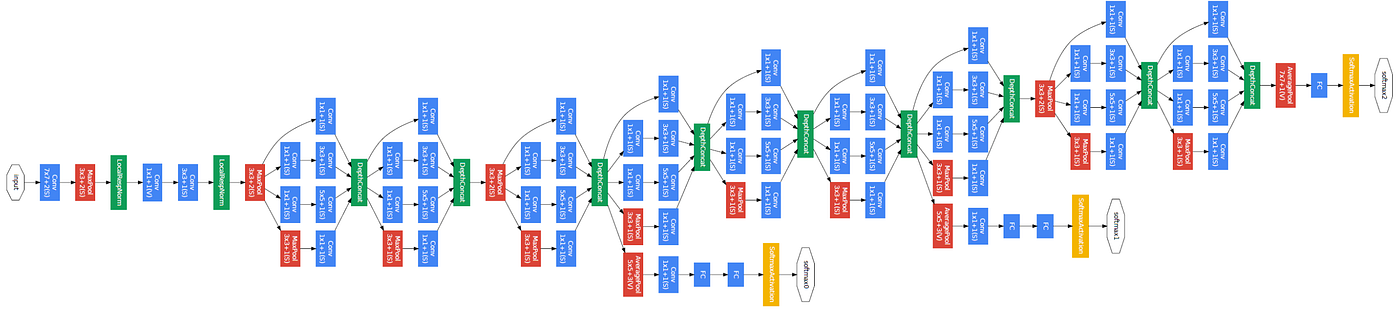
\includegraphics[width=0.45\linewidth]{img/CNN/GoogLeNet.png}
              \caption{GoogLeNet}
              \label{fig:GoogLeNet}
          \end{figure}
    \item \textbf{ResNet} is a network type that uses the idea of \textbf{residue}.
          The basic concept is to provide in input the identity function and let
          the network learn how to modify this function to approach the one you
          want to learn. The identity function is used because it can be easily
          implemented by adding the input to the result obtained at a particular
          point in the network. This is done to limit the vanishing gradient
          problem as the derivative of the identical function is always 1. With
          this trick you can implement much deeper networks.
          \begin{figure}[!ht]
              \centering
              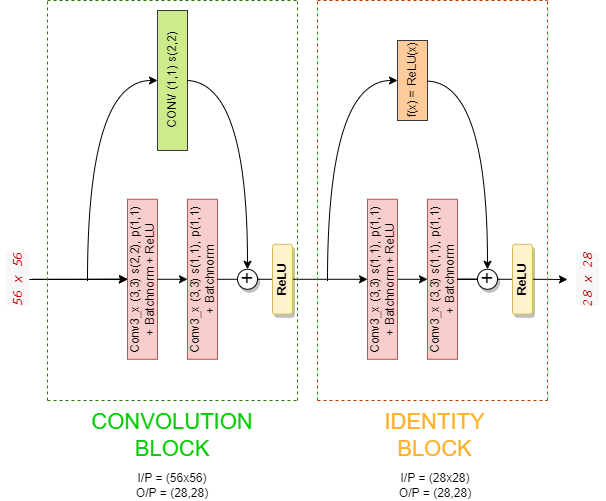
\includegraphics[width=0.45\linewidth]{img/CNN/ResNet.png}
              \caption{ResNet}
              \label{fig:resnet}
          \end{figure}
\end{itemize}

\begin{note}
    Usually we can use $1 \times 1$ convolution to squeeze information in depth
    channel without having impact on the spatial information.
\end{note}

\subsection{Transfert learning}
As mentioned above, it is not always possible to train a CNN from scratch. Depending on
the situation and the amount of data available. Generally we can train model from
scratch on a big dataset, then we can fine tune on our task dataset. In general,
one of the following techniques may be adopted:
\begin{itemize}
    \item New dataset is small and similar to original dataset: we can train a
          linear classifier on CNN features from higher layers;
    \item New dataset is large and similar to original dataset: we can Fine-tune
          the CNN;
    \item New dataset is small but very different from original dataset: we can
          train a linear classifier on CNN features from lower layers because we
          have to learn general features;
    \item New dataset is large and very different from original dataset: we can
          train CNN from scratch or fine-tune it
\end{itemize}